\documentclass[12pt, a4paper]{article}  

\usepackage{etex} % расширение классического tex в частности позволяет подгружать гораздо больше пакетов, чем мы и займёмся далее

%%%%%%%%%% Математика %%%%%%%%%%
\usepackage{amsmath,amsfonts,amssymb,amsthm,mathtools} 
%\mathtoolsset{showonlyrefs=true}  % Показывать номера только у тех формул, на которые есть \eqref{} в тексте.
%\usepackage{leqno} % Нумерация формул слева


%%%%%%%%%%%%%%%%%%%%%%%% Шрифты %%%%%%%%%%%%%%%%%%%%%%%%%%%%%%%%%
\usepackage{fontspec}         % пакет для подгрузки шрифтов
\setmainfont{HelveticaNeueCyr}   % задаёт основной шрифт документа

% why do we need \newfontfamily:
% http://tex.stackexchange.com/questions/91507/
\newfontfamily{\cyrillicfonttt}{HelveticaNeueCyr}
\newfontfamily{\cyrillicfont}{HelveticaNeueCyr}
\newfontfamily{\cyrillicfontsf}{HelveticaNeueCyr}
% Иногда тех не видит структуры шрифтов. Эти трое бравых парней спасают ситуацию и доопределяют те куски, которые Тех не увидел.

\usepackage{unicode-math}     % пакет для установки математического шрифта
\setmathfont{Asana Math}      % шрифт для математики

\usepackage{polyglossia}      % Пакет, который позволяет подгружать русские буквы
\setdefaultlanguage{russian}  % Основной язык документа
\setotherlanguage{english}    % Второстепенный язык документа



%%%%%%%%%% Работа с картинками %%%%%%%%%
\usepackage{graphicx}                  % Для вставки рисунков
\usepackage{graphics} 
\graphicspath{{images/}{pictures/}}    % можно указать папки с картинками
\usepackage{wrapfig}                   % Обтекание рисунков и таблиц текстом
\usepackage{subfigure}                 % для создания нескольких рисунков внутри одного


%%%%%%%%%% Работа с таблицами %%%%%%%%%%
\usepackage{tabularx}            % новые типы колонок
\usepackage{tabulary}            % и ещё новые типы колонок
\usepackage{array}               % Дополнительная работа с таблицами
\usepackage{longtable}           % Длинные таблицы
\usepackage{multirow}            % Слияние строк в таблице
\usepackage{float}               % возможность позиционировать объекты в нужном месте 
\usepackage{booktabs}            % таблицы как в книгах!  
\renewcommand{\arraystretch}{1.3} % больше расстояние между строками





% Заголовок
\author{Уютный факультатив} 
\title{Картинки и таблицы в \LaTeX}
\date{\today}

\begin{document} 

\maketitle

\section{Картинки}
\subsection{Вставка картинок}

% Для вставки рисунков используется команда:

\includegraphics{doge.png}

% Можно изменять размер рисунка с помощью необязательного аргумента. Например:

% уменьшить рисунок в два раза

\includegraphics[scale=0.5]{doge.png} 

% самостоятельно задать параметры длины и ширины

\includegraphics[height=3cm,width=10cm]{doge.png}

% Использовать функцию 'keepaspectratio'

\includegraphics[height=3cm,width=10cm,keepaspectratio]{doge.png}

% Вставить картинку размера 5/10 от ширины текста

\includegraphics[width=0.5\textwidth]{doge.png}

% Единицы измерения в LaTeX: 
% mm  миллиметры 
% cm  сантиметры
% in  дюймы
% 
% em  ширина буквы M используемого шрифта
% ex  высота бувы х используемого шрифта
% 
% \pagewidth   ширина страницы     \pageheight   высота страницы
% \textwidth   ширина текста       \textheight   высота текста
%
% \linewidth   длина текста в текущем окружении





\subsection{Нумерация картинок}

% Часто для размещения иллюстраций удобно использовать окружение:
% с - поставить рисунок в центре страницы где удобно теху  (center) 
% t - поставить рисунок где у добно теху и прижать к верху (top)
% b - поставить рисунок где удобно теху и прижать к низу   (bottom)
% h - поставить рисунок там, где он идет по тексту с нарушением всех правил верстки (here) 
% p - поставить рисунок на отдельной странице, целиком состоящей из "плавающих" рисунков и таблиц
% h! - поставить ну прям с высокой вероятностью там где надо нам
% H - в 100 случаях из 100 рисунок будет там где нам надо (нужен пакет float)

\begin{figure}[H]
%\caption{Заголовок мог быть и здесь}
\begin{center}

\includegraphics[width=0.3\textheight]{doge.png}
\end{center}
\caption{Картинка с изображением Doge}\label{pic:doge}
%\caption[Заголовок для списка рисунков]{Обычный заголовок}
\end{figure}

Это окружение автоматически размещает картинку в таком месте куда она входит целиком, если не указать [H].  На рис. \ref{pic:doge} изображена знаменитая собака породы хаски!


% Можно создать несколько рисунков внутри одного!
\subsection{Два рисунка внутри одного}

\begin{figure}[h!]
\begin{minipage}[h!]{0.49\linewidth} % Обратите внимание на \linewidth-длину текста в теущем окружении!
\center{\footnotesize{растровый и векторный} \\ 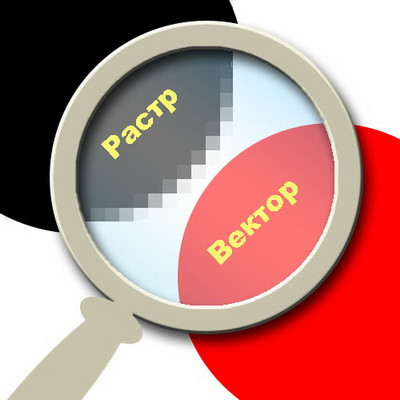
\includegraphics[width=0.8\linewidth]{rv.jpg}}
\end{minipage}
\hfill
\begin{minipage}[h!]{0.49\linewidth}
\center{\footnotesize{DOGE} \\ 
\includegraphics[width=0.8\linewidth]{doge.png}}
\end{minipage}
\caption{Две картиночки :з}
\label{fig:1figs}
\end{figure}




\section{Таблицы}

\subsection{Рисование таблиц}

%Поэкспериментировать на этой таблице с l,r hline и палочками!
\begin{tabular}{|c|c|c|c|c|c|}
\hline
$X$ & -2 & -1 & 0 & 1 & 2 \\
\hline
$P(\ldots)$ & 0.1 & 0.2 & 0.4 & 0.2 & 0.1 \\
\hline
\end{tabular}

% & разделяют столбцы, а \\ разделяют строки, \hline - прорисовка линии!


% c - колонка выровнена по центру
% l - колонка выровнена по левому краю
% r - колонка выровнена по правому краю
% p{...} - колнка верстается как абзац, в скобках - ширина колонки
% m{...} - абзац будет выровнен по середине своей высоты (лежит в array)
% b{...} - абзац будет выроавнен по нижней строке        (лежит в array)

\vspace{20mm}

\begin{tabular}{|m{3cm}|p{1cm}|p{3cm}|}
\hline
$Y$ & -1 & 0 \\
\hline
$P(\ldots)$ & 0.2 & 0.8 \\
\hline
\end{tabular}

\vspace{20mm}

% Таблицы из пакетов tabularx и tabulary работают поприятнее! Выравнивание делается так, чтобы текст занял одинаковое число строчек!

\begin{tabularx}{\textwidth}{|X|c|X|}
	\hline
	Это очень-очень длинное предложение из многих слов & Текст покороче & Это очень-очень длинное предложение из многих слов Это очень-очень длинное предложение из многих слов \\
	\hline
\end{tabularx}

% Новый формат столбцов из tabularx:
% X - подбирает столбцы равной ширины

\vspace{20mm}


\begin{tabulary}{\textwidth}{|C|J|L|}
	\hline
	Это очень-очень длинное предложение из многих слов & Текст покороче & Это очень-очень длинное предложение из многих слов Это очень-очень длинное предложение из многих слов \\
	\hline
\end{tabulary}

% Новые форматы столбцов из tabulary:
% C - выравнивание по центру
% J - выравнивание по ширине
% R - выравнивание по правому краю 
% L - выравнивание по левому краю 


\subsection{Нумерация таблиц}

В таблице \ref{tab:random} приведено распределение случайной величины $X$.

\begin{table}[h!]
\begin{center}
\begin{tabular}{|c|c|c|c|c|c|}
\hline
$X$ & -2 & -1 & 0 & 1 & 2 \\
\hline
$P(\ldots)$ & 0.1 & 0.2 & 0.4 & 0.2 & 0.1 \\
\hline
\end{tabular}
\caption{Распределение случайной величины $X$}\label{tab:random}
%\caption[Заголовок для списка таблиц]{Обычный заголовок}
\end{center}
\end{table}




\section{Объединение ячеек}

\begin{center}
\begin{tabular}{ |l|c|c| }
\hline
 & \multicolumn{2}{|c|}{Способ выбора} \\
\cline{2-3}
 & Без повторений & С повторениями  \\ \hline
\multirow{3}{*}{Порядок не важен}
                & & \\
                & $ C_n^{k} = \frac{n!}{k!(n-k)!} $ & $ \hat{C_n^k} = C_{n+k-1}^k $ \\
                & & \\

\hline
\multirow{3}{*}{Порядок важен}
               & & \\
               & $ A_n^{k} = n \cdot (n-1) \ldots \cdot (n-k+1) $ & $ \hat{A_n^k} = n^k $ \\
               & & \\
\hline
\end{tabular}
\end{center}




\subsection{Длинная таблица}

\begin{center}
\begin{longtable}{|l|l|l|}
\caption{Простая длинная таблица} \label{tab:long} \\
\hline
\textbf{First column} & \textbf{Second column} & \textbf{Third column} \\ \hline 
\endfirsthead

\multicolumn{3}{c}{\tablename{} \thetable{} --- продолжение } \\
\hline 
\textbf{First column}&\textbf{Second column} & \textbf{Third column} \\
\hline 
\endhead

\hline
\multicolumn{3}{|c|}{Продолжение на следующей странице} \\ \hline
\endfoot
\hline
\endlastfoot


One & abcdef ghjijklmn & 123.456778 \\
One & abcdef ghjijklmn & 123.456778 \\
One & abcdef ghjijklmn & 123.456778 \\
One & abcdef ghjijklmn & 123.456778 \\
One & abcdef ghjijklmn & 123.456778 \\
One & abcdef ghjijklmn & 123.456778 \\
One & abcdef ghjijklmn & 123.456778 \\
One & abcdef ghjijklmn & 123.456778 \\
One & abcdef ghjijklmn & 123.456778 \\
One & abcdef ghjijklmn & 123.456778 \\
One & abcdef ghjijklmn & 123.456778 \\
One & abcdef ghjijklmn & 123.456778 \\
One & abcdef ghjijklmn & 123.456778 \\
One & abcdef ghjijklmn & 123.456778 \\
One & abcdef ghjijklmn & 123.456778 \\
One & abcdef ghjijklmn & 123.456778 \\
One & abcdef ghjijklmn & 123.456778 \\
One & abcdef ghjijklmn & 123.456778 \\
One & abcdef ghjijklmn & 123.456778 \\
One & abcdef ghjijklmn & 123.456778 \\
One & abcdef ghjijklmn & 123.456778 \\
One & abcdef ghjijklmn & 123.456778 \\
One & abcdef ghjijklmn & 123.456778 \\
One & abcdef ghjijklmn & 123.456778 \\
One & abcdef ghjijklmn & 123.456778 \\
One & abcdef ghjijklmn & 123.456778 \\
One & abcdef ghjijklmn & 123.456778 \\
One & abcdef ghjijklmn & 123.456778 \\
One & abcdef ghjijklmn & 123.456778 \\
One & abcdef ghjijklmn & 123.456778 \\
One & abcdef ghjijklmn & 123.456778 \\
One & abcdef ghjijklmn & 123.456778 \\
One & abcdef ghjijklmn & 123.456778 \\
One & abcdef ghjijklmn & 123.456778 \\
One & abcdef ghjijklmn & 123.456778 \\
One & abcdef ghjijklmn & 123.456778 \\
One & abcdef ghjijklmn & 123.456778 \\
One & abcdef ghjijklmn & 123.456778 \\
One & abcdef ghjijklmn & 123.456778 \\
One & abcdef ghjijklmn & 123.456778 \\
One & abcdef ghjijklmn & 123.456778 \\
One & abcdef ghjijklmn & 123.456778 \\
One & abcdef ghjijklmn & 123.456778 \\
One & abcdef ghjijklmn & 123.456778 \\
One & abcdef ghjijklmn & 123.456778 \\
One & abcdef ghjijklmn & 123.456778 \\
One & abcdef ghjijklmn & 123.456778 \\
One & abcdef ghjijklmn & 123.456778 \\
One & abcdef ghjijklmn & 123.456778 \\
One & abcdef ghjijklmn & 123.456778 \\
One & abcdef ghjijklmn & 123.456778 \\
One & abcdef ghjijklmn & 123.456778 \\
One & abcdef ghjijklmn & 123.456778 \\
One & abcdef ghjijklmn & 123.456778 \\
One & abcdef ghjijklmn & 123.456778 \\
One & abcdef ghjijklmn & 123.456778 \\
One & abcdef ghjijklmn & 123.456778 \\
One & abcdef ghjijklmn & 123.456778 \\
One & abcdef ghjijklmn & 123.456778 \\
One & abcdef ghjijklmn & 123.456778 \\
One & abcdef ghjijklmn & 123.456778 \\
One & abcdef ghjijklmn & 123.456778 \\
One & abcdef ghjijklmn & 123.456778 \\
One & abcdef ghjijklmn & 123.456778 \\
One & abcdef ghjijklmn & 123.456778 \\
One & abcdef ghjijklmn & 123.456778 \\
One & abcdef ghjijklmn & 123.456778 \\
One & abcdef ghjijklmn & 123.456778 \\
One & abcdef ghjijklmn & 123.456778 \\
One & abcdef ghjijklmn & 123.456778 \\
One & abcdef ghjijklmn & 123.456778 \\
One & abcdef ghjijklmn & 123.456778 \\
One & abcdef ghjijklmn & 123.456778 \\
One & abcdef ghjijklmn & 123.456778 \\
One & abcdef ghjijklmn & 123.456778 \\
One & abcdef ghjijklmn & 123.456778 \\
One & abcdef ghjijklmn & 123.456778 \\
One & abcdef ghjijklmn & 123.456778 \\
One & abcdef ghjijklmn & 123.456778 \\
One & abcdef ghjijklmn & 123.456778 \\
\end{longtable}
\end{center}


\section{Обтекаемые таблицы и рисунки}

\begin{wrapfigure}{l}{0.3333\linewidth}
	
\includegraphics[width=\linewidth]{doge.png}
	\caption{Картинка с обтеканием}
\end{wrapfigure}


Dogecoin был создан программистом из Портланда Билли Маркусом. Он хотел создать криптовалюту, которая была бы ближе к большей демографической группе, а также дистанцироваться от истории Биткойна, в частности связанной с продажей наркотиков. Dogecoin был основан на существующей криптовалюте Luckycoin, которая в свою очередь была основана на Litecoin, которая основана на Биткойне. Как и в Luckycoin, размер награды за каждый блок в Dogecoin устанавливалась случайным образом. В марте 2014 года это положение было изменено и размер награды стал фиксированным. Изначально задумывалось, что размер эмиссии составит 100 млрд, но позже было объявлено, что производство dogecoin'ов будет неограниченным.

\begin{wraptable}{r}{0.5\linewidth}
\begin{center}
\begin{tabular}{|c|c|c|c|}
\hline
$Y$ & -1 & 0 & 1  \\
\hline
$P(\ldots)$ & 0.1 & 0.8 & 0.1 \\
\hline
\end{tabular}
\caption{Обтекаемая таблица}
\end{center}
\end{wraptable}

Сообщество Dogecoin неоднократно поддерживало сбор средств на благотворительность. В январе 2014 года сообщество участвовало в сборе 50 тыс долларов сборной Ямайки по бобслею для участия в Зимних Олимпийских играх 2014, которая получила квалификацию, но не обладала средствами для участия в соревнованиях. 25 марта 2014 года сообщество также собрало около 67,8 млн dogecoin (около 55 тыс долларов на тот момент), чтобы профинансировать гонщика Джоша Уайза (NASCAR Sprint Cup Series 2012). На следующих соревнованиях он будет выступать в машине с символикой Dogecoin.


\section{Список таблиц и список рисунков}

\listoffigures

\listoftables



\end{document}